
\section{A case-study on ASP modulo Difference Logic}
\label{sec:case}

In this section, we develop a propagator to extend ASP with \emph{quantifier free integer difference logic} (\IDL).
The complete source code of this propagator is available in the github repository at \url{https://github.com/potassco/clingo/tree/master/examples/clingo/dl}.

In addition to the rules introduced in Section~\ref{sec:background},
we now also support rules of form
\begin{lstlisting}[mathescape,numbers=none]
  &diff{$u$-$v$} <= $d$ :- $a_{1}$,...,$a_n$,not $a_{n+1}$,...,not $a_o$
\end{lstlisting}
where $u$ and $v$ are (regular) terms,
$d$ is an integer constant,
each $a_i$ is an atom,
and $0 \leq n \leq o$.
For simplicity, we restrict the occurrence of theory atoms to rule heads.%
\footnote{More general settings are discussed in~\cite{jakaosscscwa17a} and made available at~\url{https://potassco.org/clingo}.}
%
Hence, stable models may now also include theory atoms of form `\lstinline[mathescape,literate={\[}{\{}{1}{\]}{\}}{1}]{&diff [$u$-$v$] <= $d$}'.
%
More precisely,
for a stable model $X$, let $C_X$ be the set of \emph{difference constraints} such as $u-v \leq d$ associated with theory atoms
`\lstinline[mathescape,literate={\[}{\{}{1}{\]}{\}}{1}]{&diff [$u$-$v$] <= $d$}' in $X$
and $V_X$ be the set of all (integer) variables occurring in the difference constraints in $C_X$.
%
In our case, a stable model $X$ is then \emph{\IDL-stable},
if there is a mapping from $V_X$ to the set of integers
satisfying all constraints in $C_X$.

% --------------------------------------------------------------------------------
\lstinputlisting[float=t,mathescape=true,literate={\%\%}{}{0},escapeinside={\#(}{\#)},basicstyle={\ttfamily\small},label={prg:dl:theory},caption={Theory language and main loop for difference constraints (dl.lp)},language=clingo,firstline=1]{example/dl/dl.lp}
% --------------------------------------------------------------------------------
To allow for writing difference constraints in rule heads,
we define theory~\lstinline{dl} in lines~\ref{prg:dl:theory:begin}--\ref{prg:dl:theory:end} in Listing~\ref{prg:dl:theory},
a subset of the theory~\lstinline{lc} presented in Listing~\ref{prg:lc} in Section~\ref{sec:language}.
%
The following lines~\ref{prg:dl:theory:main:begin}--\ref{prg:dl:theory:main:end} implement a customized main function.
The difference to \clingo's regular main function is that a propagator for difference constraints is registered at the beginning;
grounding and solving then follow as usual.
%
Note that the solve function in line~\ref{prg:dl:theory:solve} takes a model callback as argument.
Whenever an \IDL-stable model $X$ is found,
this callback prints the mapping satisfying the corresponding difference constraints~$C_X$.
The model $X$ (excluding theory atoms) is printed as part of \clingo's default output.
% --------------------------------------------------------------------------------
\begin{figure}[t]
\centering
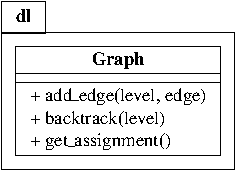
\includegraphics[]{figures/graph-interface}
\caption{Class diagram for the graph class\label{fig:class:graph}}
\end{figure}
% --------------------------------------------------------------------------------

Our exemplary propagator implements the algorithm presented in~\cite{cotmal06a}.
%
The idea is that deciding whether a set of difference constraints is satisfiable can be mapped to a graph problem.
Given a set of difference constraints, let $(V,E)$ be the weighted directed graph
where $V$ is the set of variables occurring in the constraints,
and $E$ the set of edges $(u, v, d)$ for each constraint $u-v\leq d$.
The set of difference constraints is satisfiable if the corresponding graph does not contain a negative cycle.
%
The \code{Graph} class whose interface is given in Figure~\ref{fig:class:graph} is in charge of cycle detection.
We refrain from giving the code of the \code{Graph} class and rather concentrate on describing its interface:
\begin{itemize}
\item
  Function \codeClass{Graph}{add\_edge} adds an edge of form \lstinline{(u,v,d)} to the graph. 
  If after adding the edge to the graph there is a negative cycle,
  the function returns the cycle in form of a list of edges;
  otherwise, it returns \lstinline{None}.
  Furthermore, each edge added to the graph is associated with a decision level%
  \footnote{The assignment maintains the decision level; 
    it is incremented for each decision made and decremented for each decision undone while backjumping; 
    initially, the decision level is zero.}.
  This additional information is used to backtrack to a previous state of the graph,
  whenever the solver has to backtrack to recover from a conflict.
\item
  Function \codeClass{Graph}{backtrack} takes a decision level as argument.
  It removes all edges added on that level from the graph.
  For this to work, decision levels have to be backtracked in chronological order.
  Note that the CDCL algorithm in Figure~\ref{fig:cdcl} calling our propagator also backtracks decision levels in chronological order.
\item
  As a side effect, the \code{Graph} class internally maintains an assignment of integers to nodes.
  This assignment can be turned into an assignment to the variables such that the difference constraints corresponding to the edges of the graph are satisfied.
  Function \code{get\_assignment} returns this assignment in form of a list of pairs of variables and integers.
\end{itemize}

% --------------------------------------------------------------------------------
\lstinputlisting[linerange={99-146},firstnumber=99,float=tp,mathescape=true,escapeinside={\#(}{\#)},basicstyle={\ttfamily\small},label={prg:dl:propagator},caption={Propagator for difference constraints (dl.py)},language=clingo]{example/dl/dl.py}
% --------------------------------------------------------------------------------
%
We give our exemplary propagator for difference constraints in Listing~\ref{prg:dl:propagator}.
%
It implements the \code{Propagator} interface (except for \code{check}) in Figure~\ref{fig:interface} in
lines~\ref{prg:dl:propagator:init:begin}--\ref{prg:dl:propagator:undo:end},
while featuring aspects like
incremental propagation and backtracking,
solving with multiple threads, and
multi-shot solving.
Whenever the set of edges associated with the current partial assignment of a solver induces a negative cycle
and, hence, the corresponding difference constraints are unsatisfiable,
it adds a nogood forbidding the negative cycle.
%
To this end,
it maintains data structures for, given newly added edges,
detecting whether there is a conflict.
More precisely, the propagator has three data members:
\begin{enumerate}
\item
  The \code{self.\_\_l2e} dictionary in line~\ref{prg:dl:propagator:member:l2e} maps solver literals
  for difference constraint theory atoms to their corresponding edges%
  \footnote{A solver literal might be associated with multiple edges, see Footnote~\ref{fnt:solver:literals}.},
\item
  the \code{self.\_\_e2l} dictionary in line~\ref{prg:dl:propagator:member:e2l} maps edges back to solver literals,%
  \footnote{In one solving step, the \clingo{} API guarantees that a (grounded) theory atom is associated with exactly one solver literal.
  Theory grounded in later solving steps can be associated with fresh solver literals though.}
\item
  and the \code{self.\_\_state} list in line~\ref{prg:dl:propagator:member:state} stores for each solver thread its current graph
  with the edges assigned so far.
\end{enumerate}

Function \codeClass{Propagator}{init} in lines~\ref{prg:dl:propagator:init:begin}--\ref{prg:dl:propagator:init:end}
sets up watches as well as the dictionaries in \code{self.\_\_l2e} and \code{self.\_\_e2l}.
To this end,
it traverses the theory atoms over \code{diff}$/0$ in lines~\ref{prg:dl:propagator:init:loop:begin}--\ref{prg:dl:propagator:init:loop:end}.
Note that the loop simply ignores all other theory atoms making it possible to also add propagators for other theories.
%
In lines~\ref{prg:dl:propagator:init:edge:begin}--\ref{prg:dl:propagator:init:edge:end} we extract the edge from the theory atom.%
\footnote{Here we assume that the user supplied a valid theory atom.
  A propagator for production should check validity and provide proper error messages.}
%
Each such atom is associated with a solver literal,
obtained in line~\ref{prg:dl:propagator:init:map-literal}.
The mappings between solver literals and corresponding edges are then stored in the \code{self.\_\_l2e} and \code{self.\_\_e2l} dictionaries in
lines~\ref{prg:dl:propagator:init:l2e} and~\ref{prg:dl:propagator:init:e2l}.\footnote{
  \python's \code{setdefault} function is used to update the mappings.
  Depending on whether the given \code{key} already appears in the dictionary,
  the function either retrieves the associated value or inserts and returns the second argument.}
In the last line of the loop, a watch is added for each solver literal at hand,
so that the solver calls \code{propagate} whenever the edge has to be added to the graph.

Function \codeClass{Propagator}{propagate}, given in lines~\ref{prg:dl:propagator:propagate:begin}--\ref{prg:dl:propagator:propagate:end},
accesses \code{control.thread\_id} in line~\ref{prg:dl:propagator:propagate:state}
to obtain the graph associated with the active thread.
%
The loops in lines~\ref{prg:dl:propagator:propagate:loop:begin}--\ref{prg:dl:propagator:propagate:loop:end} then iterate over the list of changes and associated edges.
In line \ref{prg:dl:propagator:propagate:add-edge} each such edge is added to the graph.
If adding the edge produced a negative cycle,
a nogood is added in line~\ref{prg:dl:propagator:propagate:add-nogood}.
Because an edge can be associated with multiple solver literals,
we use function \codeClass{Propagator}{\_\_literal}
retrieving the first solver literal associated with an edge that is true,
to construct the nogood forbidding the cycle.
%
Given that the solver has to resolve the conflict and backjump,
the call to \code{add\_nogood} always yields false,
so that propagation is stopped without processing the remaining changes any further.\footnote{%
  The optional arguments \code{tag} and \code{lock} of \code{add\_nogood} can be used to control the scope and lifetime of recorded nogoods.
  Furthermore, if a propagator adds nogoods that are not necessarily violated,
  function \code{control.propagate} can be invoked to trigger unit propagation.}

Given that each edge added to the graph in line~\ref{prg:dl:propagator:propagate:add-edge} is associated with the current decision level,
the implementation of function \codeClass{Propagator}{undo} is quite simple.
It calls function \codeClass{Graph}{backtrack} on the solver's graph to remove all edges added on the current decision level.

% --------------------------------------------------------------------------------
\begin{figure}[ht]
\centering
{\def\svgscale{.4}
%% Creator: Inkscape inkscape 0.91, www.inkscape.org
%% PDF/EPS/PS + LaTeX output extension by Johan Engelen, 2010
%% Accompanies image file 'dl.pdf' (pdf, eps, ps)
%%
%% To include the image in your LaTeX document, write
%%   \input{<filename>.pdf_tex}
%%  instead of
%%   \includegraphics{<filename>.pdf}
%% To scale the image, write
%%   \def\svgwidth{<desired width>}
%%   \input{<filename>.pdf_tex}
%%  instead of
%%   \includegraphics[width=<desired width>]{<filename>.pdf}
%%
%% Images with a different path to the parent latex file can
%% be accessed with the `import' package (which may need to be
%% installed) using
%%   \usepackage{import}
%% in the preamble, and then including the image with
%%   \import{<path to file>}{<filename>.pdf_tex}
%% Alternatively, one can specify
%%   \graphicspath{{<path to file>/}}
%% 
%% For more information, please see info/svg-inkscape on CTAN:
%%   http://tug.ctan.org/tex-archive/info/svg-inkscape
%%
\begingroup%
  \makeatletter%
  \providecommand\color[2][]{%
    \errmessage{(Inkscape) Color is used for the text in Inkscape, but the package 'color.sty' is not loaded}%
    \renewcommand\color[2][]{}%
  }%
  \providecommand\transparent[1]{%
    \errmessage{(Inkscape) Transparency is used (non-zero) for the text in Inkscape, but the package 'transparent.sty' is not loaded}%
    \renewcommand\transparent[1]{}%
  }%
  \providecommand\rotatebox[2]{#2}%
  \ifx\svgwidth\undefined%
    \setlength{\unitlength}{297.11999512bp}%
    \ifx\svgscale\undefined%
      \relax%
    \else%
      \setlength{\unitlength}{\svgscale\unitlength}%
    \fi%
  \else%
    \setlength{\unitlength}{\svgwidth}%
  \fi%
  \global\let\svgwidth\undefined%
  \global\let\svgscale\undefined%
  \makeatother%
  \begin{picture}(1,0.51534733)%
    \put(0,0){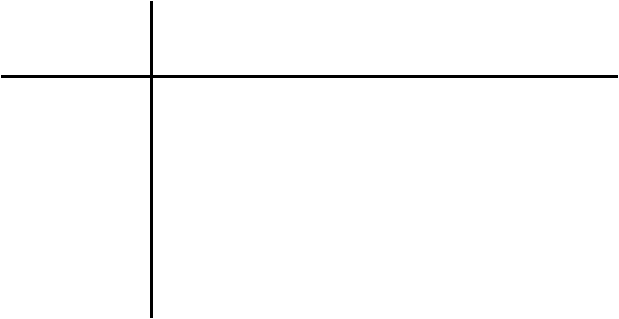
\includegraphics[width=\unitlength,page=1]{figures/dl.pdf}}%
    \put(0.20382337,0.43268764){\color[rgb]{0,0,0}\makebox(0,0)[rb]{\smash{task}}}%
    \put(0.28459882,0.43268764){\color[rgb]{0,0,0}\makebox(0,0)[lb]{\smash{duration on machine}}}%
    \put(0.20382337,0.28459932){\color[rgb]{0,0,0}\makebox(0,0)[rb]{\smash{a}}}%
    \put(0.20382337,0.16343615){\color[rgb]{0,0,0}\makebox(0,0)[rb]{\smash{b}}}%
    \put(0.20382337,0.04227298){\color[rgb]{0,0,0}\makebox(0,0)[rb]{\smash{c}}}%
    \put(0,0){\includegraphics[width=\unitlength,page=2]{figures/dl.pdf}}%
  \end{picture}%
\endgroup%
}
\caption{Flow shop: instance with three tasks and two machines\label{fig:fs:ins}}
\end{figure}
\begin{figure}[ht]
\centering
{\def\svgwidth{\linewidth}
%% Creator: Inkscape inkscape 0.91, www.inkscape.org
%% PDF/EPS/PS + LaTeX output extension by Johan Engelen, 2010
%% Accompanies image file 'dl-sol.pdf' (pdf, eps, ps)
%%
%% To include the image in your LaTeX document, write
%%   \input{<filename>.pdf_tex}
%%  instead of
%%   \includegraphics{<filename>.pdf}
%% To scale the image, write
%%   \def\svgwidth{<desired width>}
%%   \input{<filename>.pdf_tex}
%%  instead of
%%   \includegraphics[width=<desired width>]{<filename>.pdf}
%%
%% Images with a different path to the parent latex file can
%% be accessed with the `import' package (which may need to be
%% installed) using
%%   \usepackage{import}
%% in the preamble, and then including the image with
%%   \import{<path to file>}{<filename>.pdf_tex}
%% Alternatively, one can specify
%%   \graphicspath{{<path to file>/}}
%% 
%% For more information, please see info/svg-inkscape on CTAN:
%%   http://tug.ctan.org/tex-archive/info/svg-inkscape
%%
\begingroup%
  \makeatletter%
  \providecommand\color[2][]{%
    \errmessage{(Inkscape) Color is used for the text in Inkscape, but the package 'color.sty' is not loaded}%
    \renewcommand\color[2][]{}%
  }%
  \providecommand\transparent[1]{%
    \errmessage{(Inkscape) Transparency is used (non-zero) for the text in Inkscape, but the package 'transparent.sty' is not loaded}%
    \renewcommand\transparent[1]{}%
  }%
  \providecommand\rotatebox[2]{#2}%
  \ifx\svgwidth\undefined%
    \setlength{\unitlength}{948.00009766bp}%
    \ifx\svgscale\undefined%
      \relax%
    \else%
      \setlength{\unitlength}{\svgscale\unitlength}%
    \fi%
  \else%
    \setlength{\unitlength}{\svgwidth}%
  \fi%
  \global\let\svgwidth\undefined%
  \global\let\svgscale\undefined%
  \makeatother%
  \begin{picture}(1,0.45569621)%
    \put(0,0){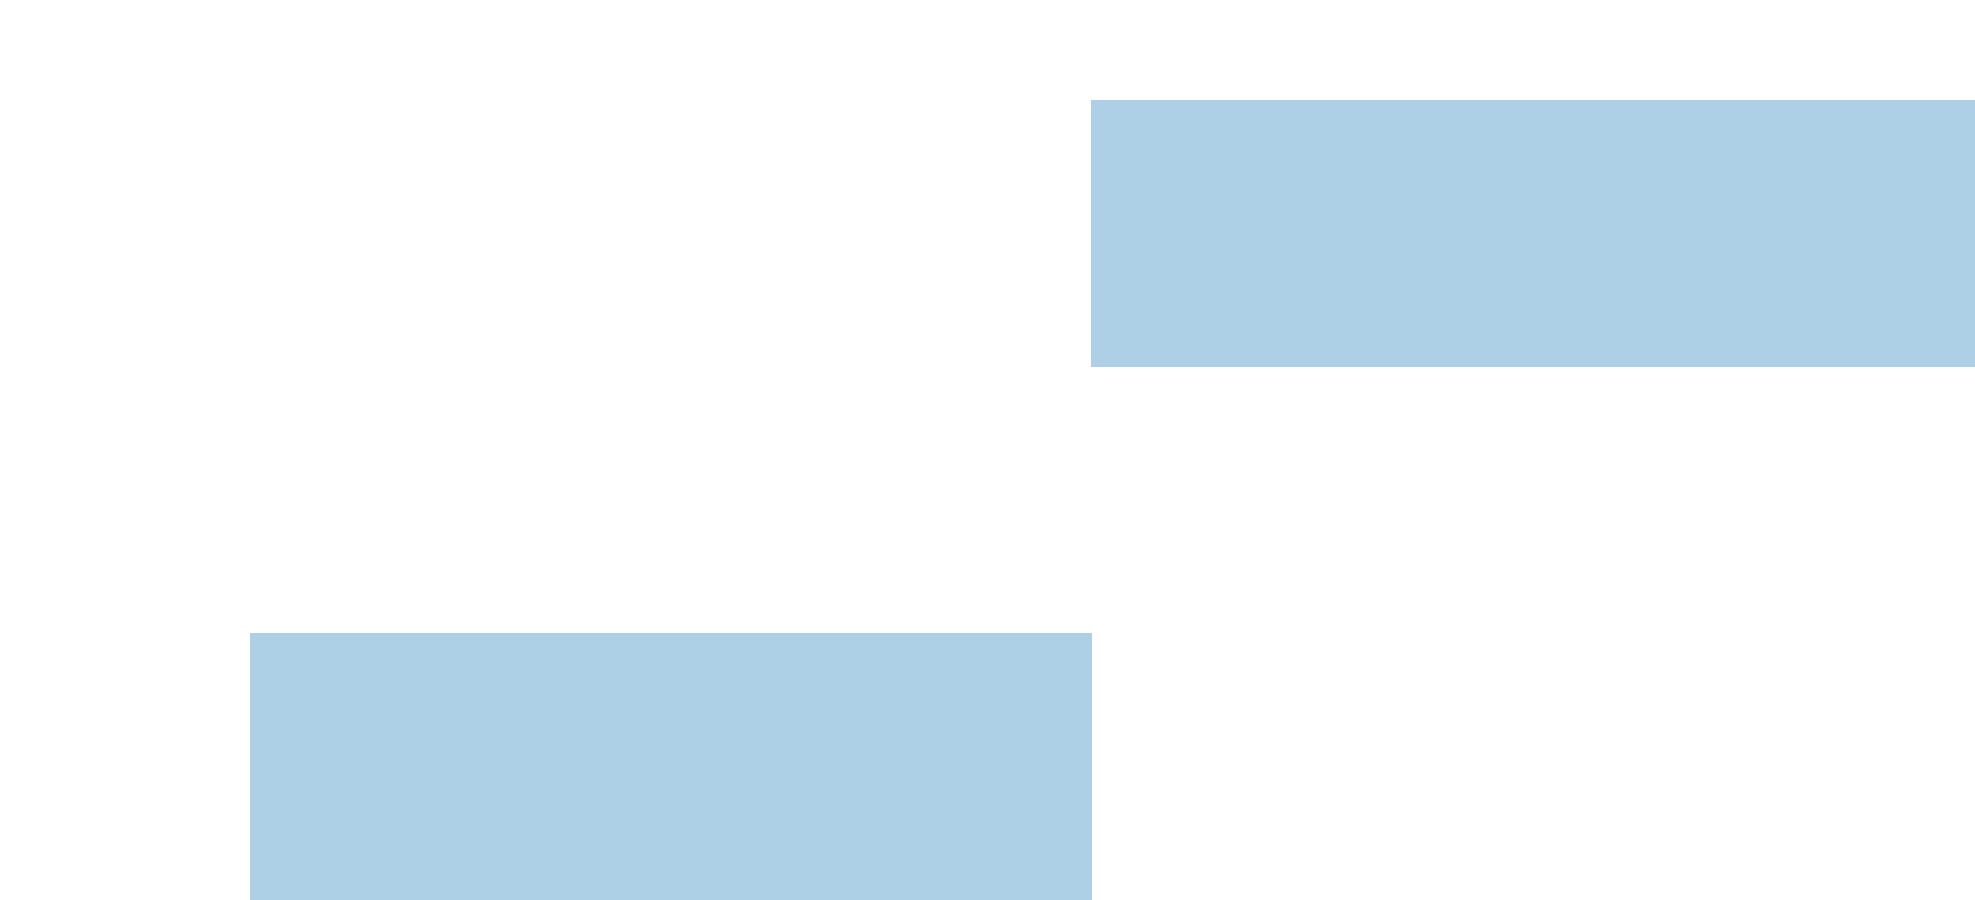
\includegraphics[width=\unitlength,page=1]{figures/dl-sol.pdf}}%
    \put(0.13924056,0.23206748){\color[rgb]{0,0,0}\makebox(0,0)[lb]{\smash{a < c < b}}}%
    \put(0,0){\includegraphics[width=\unitlength,page=2]{figures/dl-sol.pdf}}%
    \put(0.1139241,0.18565396){\color[rgb]{0,0,0}\makebox(0,0)[rb]{\smash{1}}}%
    \put(0.1139241,0.14767931){\color[rgb]{0,0,0}\makebox(0,0)[rb]{\smash{2}}}%
    \put(0,0){\includegraphics[width=\unitlength,page=3]{figures/dl-sol.pdf}}%
    \put(0.1139241,0.41772158){\color[rgb]{0,0,0}\makebox(0,0)[rb]{\smash{machine}}}%
    \put(0.13924056,0.36708866){\color[rgb]{0,0,0}\makebox(0,0)[lb]{\smash{a < b < c}}}%
    \put(0,0){\includegraphics[width=\unitlength,page=4]{figures/dl-sol.pdf}}%
    \put(0.1139241,0.32067507){\color[rgb]{0,0,0}\makebox(0,0)[rb]{\smash{1}}}%
    \put(0.1139241,0.28270039){\color[rgb]{0,0,0}\makebox(0,0)[rb]{\smash{2}}}%
    \put(0,0){\includegraphics[width=\unitlength,page=5]{figures/dl-sol.pdf}}%
    \put(0.13924056,0.41772158){\color[rgb]{0,0,0}\makebox(0,0)[lb]{\smash{solution}}}%
    \put(0,0){\includegraphics[width=\unitlength,page=6]{figures/dl-sol.pdf}}%
    \put(0.13924056,0.0970464){\color[rgb]{0,0,0}\makebox(0,0)[lb]{\smash{b < a < c}}}%
    \put(0,0){\includegraphics[width=\unitlength,page=7]{figures/dl-sol.pdf}}%
    \put(0.1139241,0.0506329){\color[rgb]{0,0,0}\makebox(0,0)[rb]{\smash{1}}}%
    \put(0.1139241,0.01265828){\color[rgb]{0,0,0}\makebox(0,0)[rb]{\smash{2}}}%
    \put(0.5696203,0.23206748){\color[rgb]{0,0,0}\makebox(0,0)[lb]{\smash{c < a < b}}}%
    \put(0,0){\includegraphics[width=\unitlength,page=8]{figures/dl-sol.pdf}}%
    \put(0.5696203,0.36708846){\color[rgb]{0,0,0}\makebox(0,0)[lb]{\smash{b < c < a}}}%
    \put(0,0){\includegraphics[width=\unitlength,page=9]{figures/dl-sol.pdf}}%
    \put(0.5696203,0.0970463){\color[rgb]{0,0,0}\makebox(0,0)[lb]{\smash{c < b < a}}}%
    \put(0,0){\includegraphics[width=\unitlength,page=10]{figures/dl-sol.pdf}}%
    \put(0.54008433,0.36708862){\color[rgb]{0,0,0}\makebox(0,0)[rb]{\smash{18}}}%
    \put(0.54008433,0.23206754){\color[rgb]{0,0,0}\makebox(0,0)[rb]{\smash{19}}}%
    \put(0.54008433,0.09704645){\color[rgb]{0,0,0}\makebox(0,0)[rb]{\smash{16}}}%
    \put(0.98734167,0.36708862){\color[rgb]{0,0,0}\makebox(0,0)[rb]{\smash{16}}}%
    \put(0.98734167,0.23206754){\color[rgb]{0,0,0}\makebox(0,0)[rb]{\smash{20}}}%
    \put(0.98734167,0.09704645){\color[rgb]{0,0,0}\makebox(0,0)[rb]{\smash{20}}}%
  \end{picture}%
\endgroup%
}
\caption{Flow shop: solutions for all possible permutations with the total execution length in the top right corner and optimal solutions with a blue background\label{fig:fs:sol}}
\end{figure}
% --------------------------------------------------------------------------------
%
To see our propagator in action, we consider the flow shop problem,
dealing with a set of tasks $T$ that have to be consecutively executed on $m$ machines.
%
Each task has to be processed on each machine from $1$ to $m$. 
Different parts of one task are completed on each machine resulting in the completion of the task after execution on all machines is finished.
Before a task can be processed on machine $i$, it has to be finished on machine $i-1$.
The duration of different tasks on the same machine may vary.
A task can only be executed on one machine at a time and
a machine must not be occupied by more than one task at a time.
%
An (optimal) solution to the problem is a permutation of tasks so that all tasks are finished as early as possible.

Figure~\ref{fig:fs:ins} depicts a possible instance for the flow shop problem.
The three tasks \code{a}, \code{b}, and \code{c} have to be scheduled on two machines.
The colored boxes indicate how long a task has to run on a machine.
Lighter shades of the same color are for the first and darker ones for the second machine.
For example, task \code{a} needs to be processed for~$3$ time units on the first and~$4$ time units on the second machine.

% --------------------------------------------------------------------------------
\lstinputlisting[float=ht,mathescape=true,escapeinside={\#(}{\#)},basicstyle={\ttfamily\small},label={prg:fs:ins},caption={Flow shop instance (fsI.lp)},language=clingo]{example/dl/fsI.lp}
% --------------------------------------------------------------------------------
\lstinputlisting[float=ht,literate={\%\%}{}{0},linerange={1-21,23-24},mathescape=true,escapeinside={\#(}{\#)},basicstyle={\ttfamily\small},label={prg:fs:enc},caption={Encoding of flow shop using difference constraints (fsE.lp)},language=clingo]{example/dl/fsE.lp}
% --------------------------------------------------------------------------------
%
Next we encode this problem using difference constraints.
We give in Listing~\ref{prg:fs:ins} a straightforward encoding of the instance in Figure~\ref{fig:fs:ins}.
Listing~\ref{prg:fs:enc} depicts the encoding of the flow shop problem.
Following the generate, define, and test methodology of ASP,
we first generate in lines~\ref{prg:fs:perm:begin}--\ref{prg:fs:perm:end} all possible permutations of tasks,
where atoms of form \code{permutation(T,U)} encode that task~$T$ has to be executed before task~$U$.
Then, in the following lines~\ref{prg:fs:diff:begin}--\ref{prg:fs:diff:end},
we use difference constraints to calculate the duration of the generated permutation.
%
The difference constraint in line~\ref{prg:fs:permutation:seq} guarantees that the tasks are executed in the right order.
For example, $\code{(a,1)} - \code{(a,2)} \leq -d$ ensures that task~\code{a} can only be executed on machine~\code{2} if it has finished on machine~\code{1}.
Hence, variable \code{(a,2)} has to be assigned so that it is greater or equal to $\code{(a,2)}-d$ where $d$ is the duration of task \code{a} on machine \code{1}.
Similarly, $\code{(a,1)} - \code{(b,1)} \leq -d$ makes sure that task~\code{b} can only be executed on machine~\code{1} if task~\code{a} has finished on machine~\code{1}.
While the first constraint is a fact (see line~\ref{prg:fs:permutation:seq:machine}),
the latter is subject to the generated permutation of tasks (see line~\ref{prg:fs:permutation:seq:task}).
%
The difference constraint in line~\ref{prg:fs:null} ensures that all time points at which a task is started are greater than zero.
Note that this constraint is in principle redundant
but since sets of difference constraints always have infinitely many solutions
it is good practice to encode relative to a starting point.
Furthermore, note that~\code{0} is actually a variable.
In fact, the \code{Graph} class takes care of subtracting the value of variable~\code{0} from all other variables when returning an assignment
to get easier interpretable solutions.

Running encoding and instance with the \code{dl} propagator results in the following $6$ solutions
corresponding to the solutions in Figure~\ref{fig:fs:sol}.%
\footnote{Note that in each solution all tasks are executed as early as possible.
  This is no coincidence and actually guaranteed by the algorithm implemented in the \code{Graph} class.}
One for each possible permutation of tasks:
%
% --------------------------------------------------------------------------------
\lstinputlisting[numbers=none,escapechar=!,basicstyle={\ttfamily\small}]{example/dl/fsA.txt}
% --------------------------------------------------------------------------------

% --------------------------------------------------------------------------------
\lstinputlisting[float=tp,mathescape=true,literate={\%\%}{}{0},escapeinside={\#(}{\#)},basicstyle={\ttfamily\small},label={prg:dl:theory:opt},caption={Main loop for difference constraints with optimization (dlO.lp)},language=clingo,firstline=1]{example/dl/dlO.lp}
% --------------------------------------------------------------------------------
%
Finally, to find optimal solutions,
we combine the algorithms in Listing~\ref{prg:opt:main} and Listing~\ref{prg:dl:theory} to minimize the total execution time of the tasks.
The adapted algorithm is given in Listing~\ref{prg:dl:theory:opt} .
%
As with algorithm in~\ref{prg:dl:theory}, a propagator is registered before solving.
And the control flow is similar to the branch-and-bound-based optimization algorithm in Listing~\ref{prg:opt:main}
except that we now minimize the variable \code{bound};
or better the difference between variable~\code{0} and~\code{bound}
by adding the difference constraint $\code{0} - \code{bound} \leq b$ to the program in line~\ref{prg:dl:theory:opt:bound}
where $b$ is the best known execution time of the tasks as obtained from the assignment in line~\ref{prg:dl:theory:opt:get-bound} minus $1$.
To bound maximum execution time of the task,
we have to add one more line to the encoding in Listing~\ref{prg:fs:enc}:
\begin{lstlisting}[language=clingo,firstnumber=22]
  &diff { (T,M)-bound } <= -D :- duration(T,M,D).
\end{lstlisting}
This makes sure that each task ends within the given bound.
Running encoding and instance with the \code{dl} propagator results in the optimum bound~$16$ where
the obtained solution corresponds to the left of the two optimal solutions indicated by a light blue background in Figure~\ref{fig:fs:sol}:
% --------------------------------------------------------------------------------
\lstinputlisting[numbers=none,escapechar=!,basicstyle={\ttfamily\small}]{example/dl/fsO.txt}
% --------------------------------------------------------------------------------

%%% Local Variables:
%%% mode: latex
%%% TeX-master: "paper"
%%% End:
